% diagrams/lineas-circulo.tex -- un círculo y dos trazos sueltos,
% deliberadamente SIN forma reconocible, para la actividad "Completa": la
% niña los convierte en su propio dibujo (una cara, un sol, un globo, una
% flor, una rueda... lo que se le ocurra).
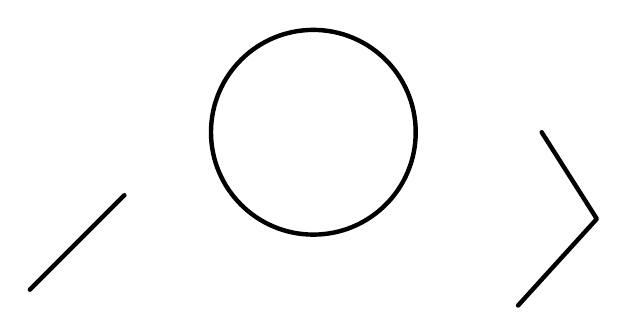
\begin{tikzpicture}[line width=1.6pt, line cap=round, line join=round]
  \draw (0,-0.6) circle (1.3);
  \draw (-3.6,-2.6) -- (-2.4,-1.4);
  \draw (2.6,-2.8) -- (3.6,-1.7) -- (2.9,-0.6);
\end{tikzpicture}
